\section{Prototype}
\subsection{Model}
Ud fra vores vision om et receptfornyelsesmodul, vores udarbejdede user stories og vores MoSCoW prioriteringer har vi udviklet nedenstående ER-diagram over vores domæne.\\
\missingfigure{ER diagram}\\
Vores recept entitet kan unikt identificeres ud fra vores andre entiteters nøgler, og er derfor lavet en weak entity. Blandt vores ønskede funktioner er historik og medicinkort. Da der i en log over historik godt kan fremstå den samme medicin til den samme patient flere gange, har det været nødvendigt at tilføje en 'Historik' entitet som udover ovennævnte kan holde tidspunktet for fornyelsen af recepten.\\
Medicinkortet kan 'laves' ud fra recept entiteten givet hvilken patient der ønsker at se sit medicinkort. Det har derfor ikke været nødvendigt at lave en entitet til denne feature.\\

Vi har herefter omsat vores entiteter til tabeller på samme hvis som beskrevet i \textit{'Database Systems. The Complete Book'}\footnote{Prentice Hall, Database Systems. The Complete Book, s. 157-163}. Mange af vores entiteter kan laves direkte til en tabeller som ses nedenfor:
\begin{align*}
	&\textrm{Patient}(\textrm{\underline{CPR}, Password})\\
	&\textrm{Apotek}(\textrm{\underline{Navn}, Addresse})\\
	&\textrm{Medicin}(\textrm{\underline{Navn}, \underline{Styrke}})\\
\end{align*}
Ligeledes kan 'Diagnose' laves direkte. Denne tabel vil komme til at indeholde alle de diagnoser som kan gives, og er nødvendig da en patient kan have mere end en diagnose.\todo{High potential for change}
\begin{equation*}
\textrm{Diagnose}(\textrm{\underline{Sygdom}})
\end{equation*}
Vi har herefter vores 'Recept' entitet. Denne er weak, og henter nøgler fra de fleste andre entiteter. 'Status' attributten vil blive benyttet i overensstemmelse med vores vision om at patienten selv skal kunne følge med i receptfornyelsesprocessen. 'Udstedt' attributten vil blive benyttet af medicinkortet, og vil aldrig ændre sig da den repræsenterer hvornår patienter første gang blev ordineret med medicinen. 'Udløber' attributten vil blive benyttet til at sende reminders til patienterne.\todo{For detaljeret? Nogen grund til at forklare disse attributter?} 
\begin{equation*}
	\textrm{Recept}(\textrm{\underline{ApoNavn}, \underline{MedNavn}, \underline{MedStyrke}, \underline{PatCPR}, \underline{fornyet}, status, udstedt, udløber})
\end{equation*}
Hvis vi skulle lave vores relationer til om til tabeller ville der blive en en masse redundancy da alle på nær en enkelt relation vil allerede være subsets af andre tabeller. Derfor er den eneste relation som bliver lavet om til en tabel 'Behandles for'. Her vil begge nøgler være foreign keys til henholdsvis 'Patient' og 'Dignose'.
\begin{equation*}
\textrm{BehandlesFor}(\textrm{\underline{PatCPR}, \underline{Sygdom}})
\end{equation*}
\subsection{Prototype Flask}
Vores Flask applikation tager udgangspunkt i \textit{'prototype/\_\_init\_\_.py'} hvor oplysningerne om vores database er sat på linje 8. Det er også i denne fil vores blueprint 'Main' bliver registreret. Vi har også defineret en commandline command 'test' som kører vores tests.\\
I filen \textit{'prototype/models.py'} er der lavet klasser over de af vores tabeller som vi benytter i vores prototype. Dette gør at vi kan skrive queries som henter en række ned fra vores database og lave et objekt over oplysningerne. Det er også i denne fil vi har defineret vores queries som metoder.\\
I filen \textit{'prototype/Main/routes.py'} finder vi vores routes som definerer de sider vores prototype benytter. De mest interessante er \textit{'/receptfornyelse'}, \textit{'/renew/<med\_name>/<med\_conc>'} og \textit{'/login'}. Disse sider benytter før nævnte objekter og queries til at udføre vores business logic før siderne bliver renderet. Vores 'receptfornyelse' route kører vores \textit{'get\_Active\_Prescriptions'} query for at finde brugerens aktive recepter. Resultatet af denne query er en liste af 'Prescription' objekter som bliver givet videre til vores view der itererer over alle objekterne i listen for at skabe en dynamisk webside. Vores '/renew/<med\_name>/<med\_conc>' route bliver besøgt fra vores receptfornyelses side når brugeren klikker for at fornye sin recept. Denne route sørger for at den tidligere aktive recept bliver gjort inaktiv, og at der bliver lavet en ny recept som bliver den aktive.\\
I filen \textit{'prototype/tests/test\_model.py'} findes vores tests som kan køres som beskrevet nedenfor.

\subsection{Tests}
For at eliminere de værste fejl i vores protorype har vi valgt at skrive unit tests til alle vores queries defineret i \textit{models.py}. Disse kan køres med \textit{Flask test} fra kommandolinjen hvis ens 'FLASK\_APP' environment variable er sat til 'prototype.py', og man befinder sig i rod mappen. Vores tests kan også køres fra roden med kommandoen 'python -m unittest prototype/tests/test\_model.py'.\\
Vores tests forudsætter at der er sat en testdatabase op ved navn 'prototypetests'.
\newpage
\subsection{Showcasing af prototype}
Vores prototype kan køres med \textit{Flask run} fra kommandolinjen hvis ens 'FLASK\_APP' environment variable er sat til 'prototype.py', og man befinder sig i rod mappen. Vores prototype kan også køres fra roden med kommandoen 'python prototype.py'.\\
Vores prototype forudsætter at der er sat en database op ved navn 'prototype'.

\begin{figure}[h!]
	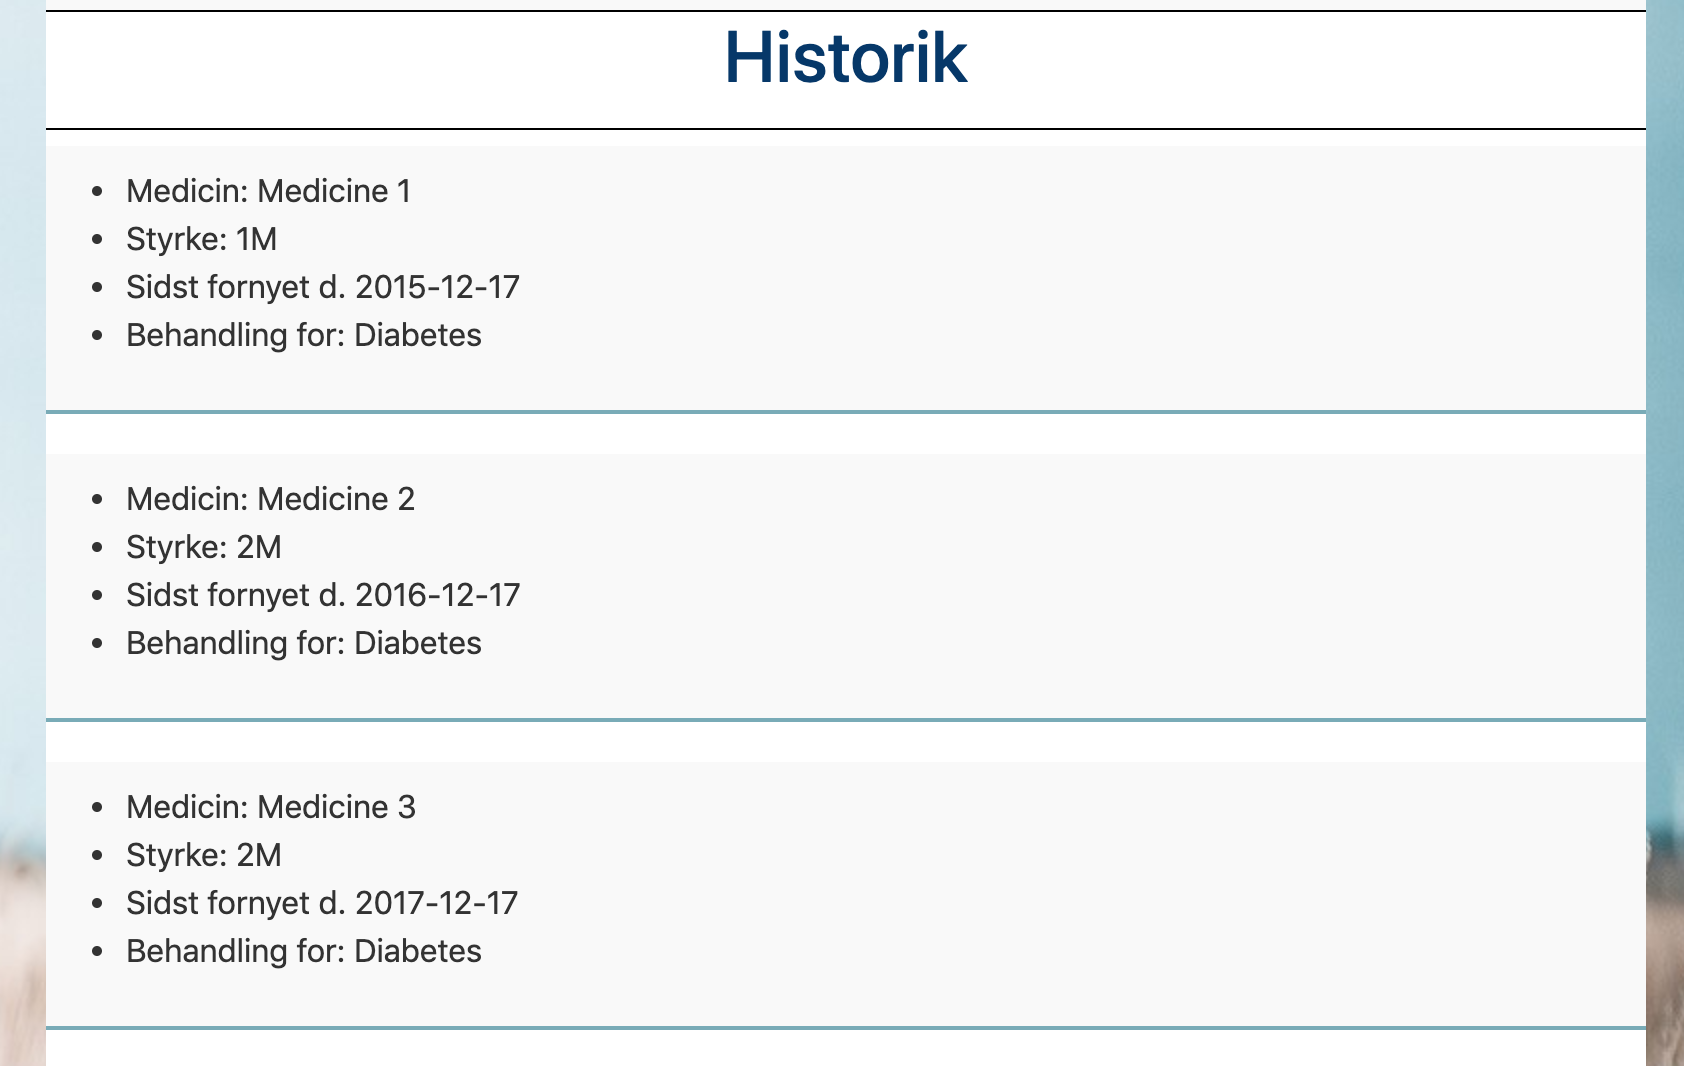
\includegraphics[width=\linewidth]{Materials/Prototype/Historik}
	\caption{Historik for en bruger}
\end{figure}

Vores prototype består hovedsagligt af tre funktionaliteter: \textit{Receptfornyelse, Historik} og \textit{Sundhedsdata}. Under \textit{Historik} er det muligt at se alle ens recepter og tidligere recepter, samt information omkring hvornår recepten blev udskrevet, hvornår den udløb og hvilken medicin der blev udskrevet.\\
Under \textit{Receptfornyelse} kan alle ens aktive recepter ses. Øverst på siden er en processlinje som beskriver hvor langt i 'forløbet' ens medicin er kommet, altså er medicinen først lige bestilt? Har lægen godkendt receptfornyelsen? Kan medicinen afhentes? Denne processlinje understøtter vores vision om at brugeren skal indrages i forløbet, og selv kan se fremskridtene i processen. Nedenunder ses de aktive recepter samt en knap som tillader at fornye recepten. Når brugeren klikker forny ud fra en af sine recepter, så opdateres recepten til ikke længere at være aktiv, og der bliver i stedet lavet en ny recept. I prototypen er de fleste af værdierne i den nye recept hard coded, men dette ville nemt kunne gøres mere realistisk ved at lave om i vores database model.
\begin{figure}[h!]
	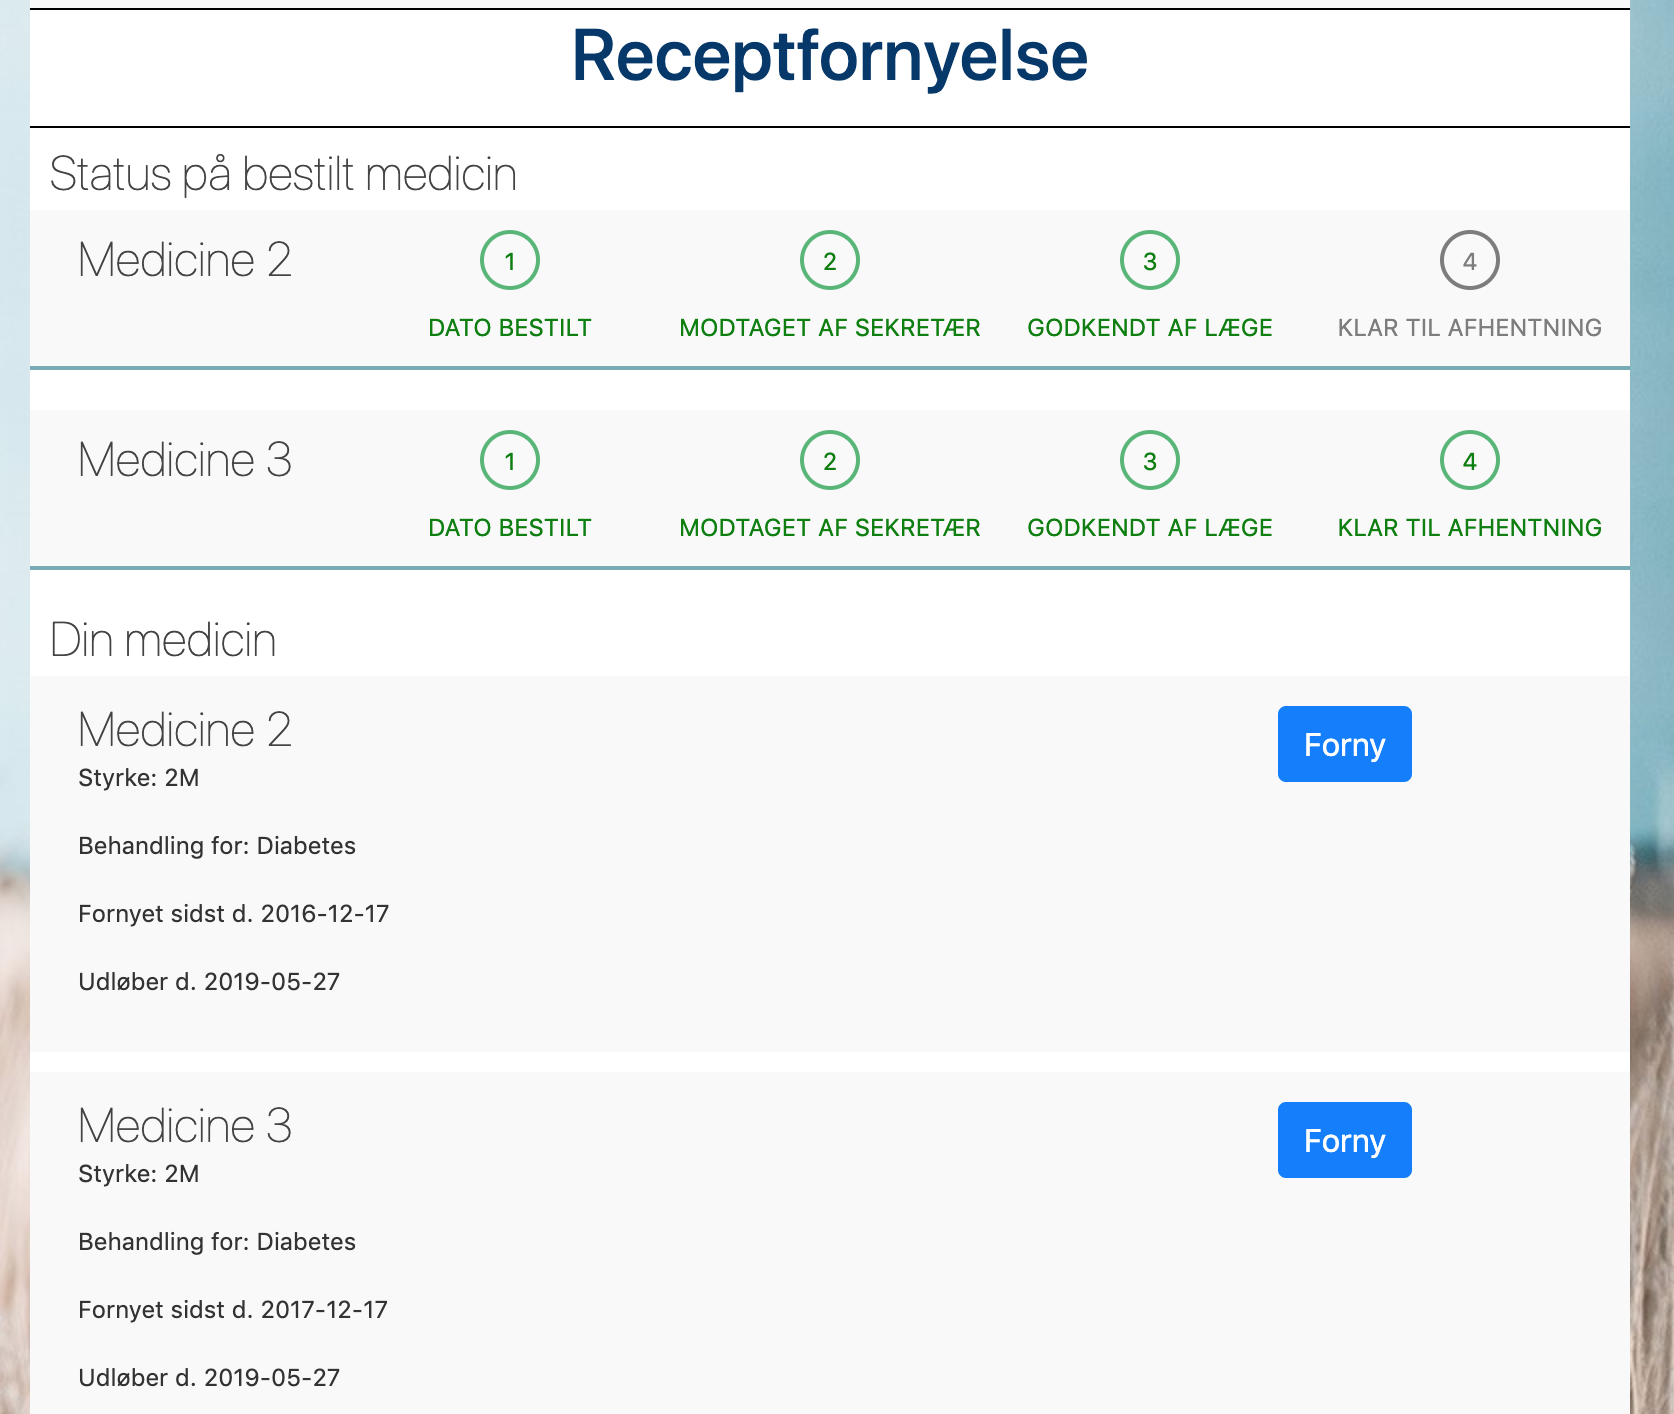
\includegraphics[width=0.49\linewidth]{Materials/Prototype/Receptfornyelse}
	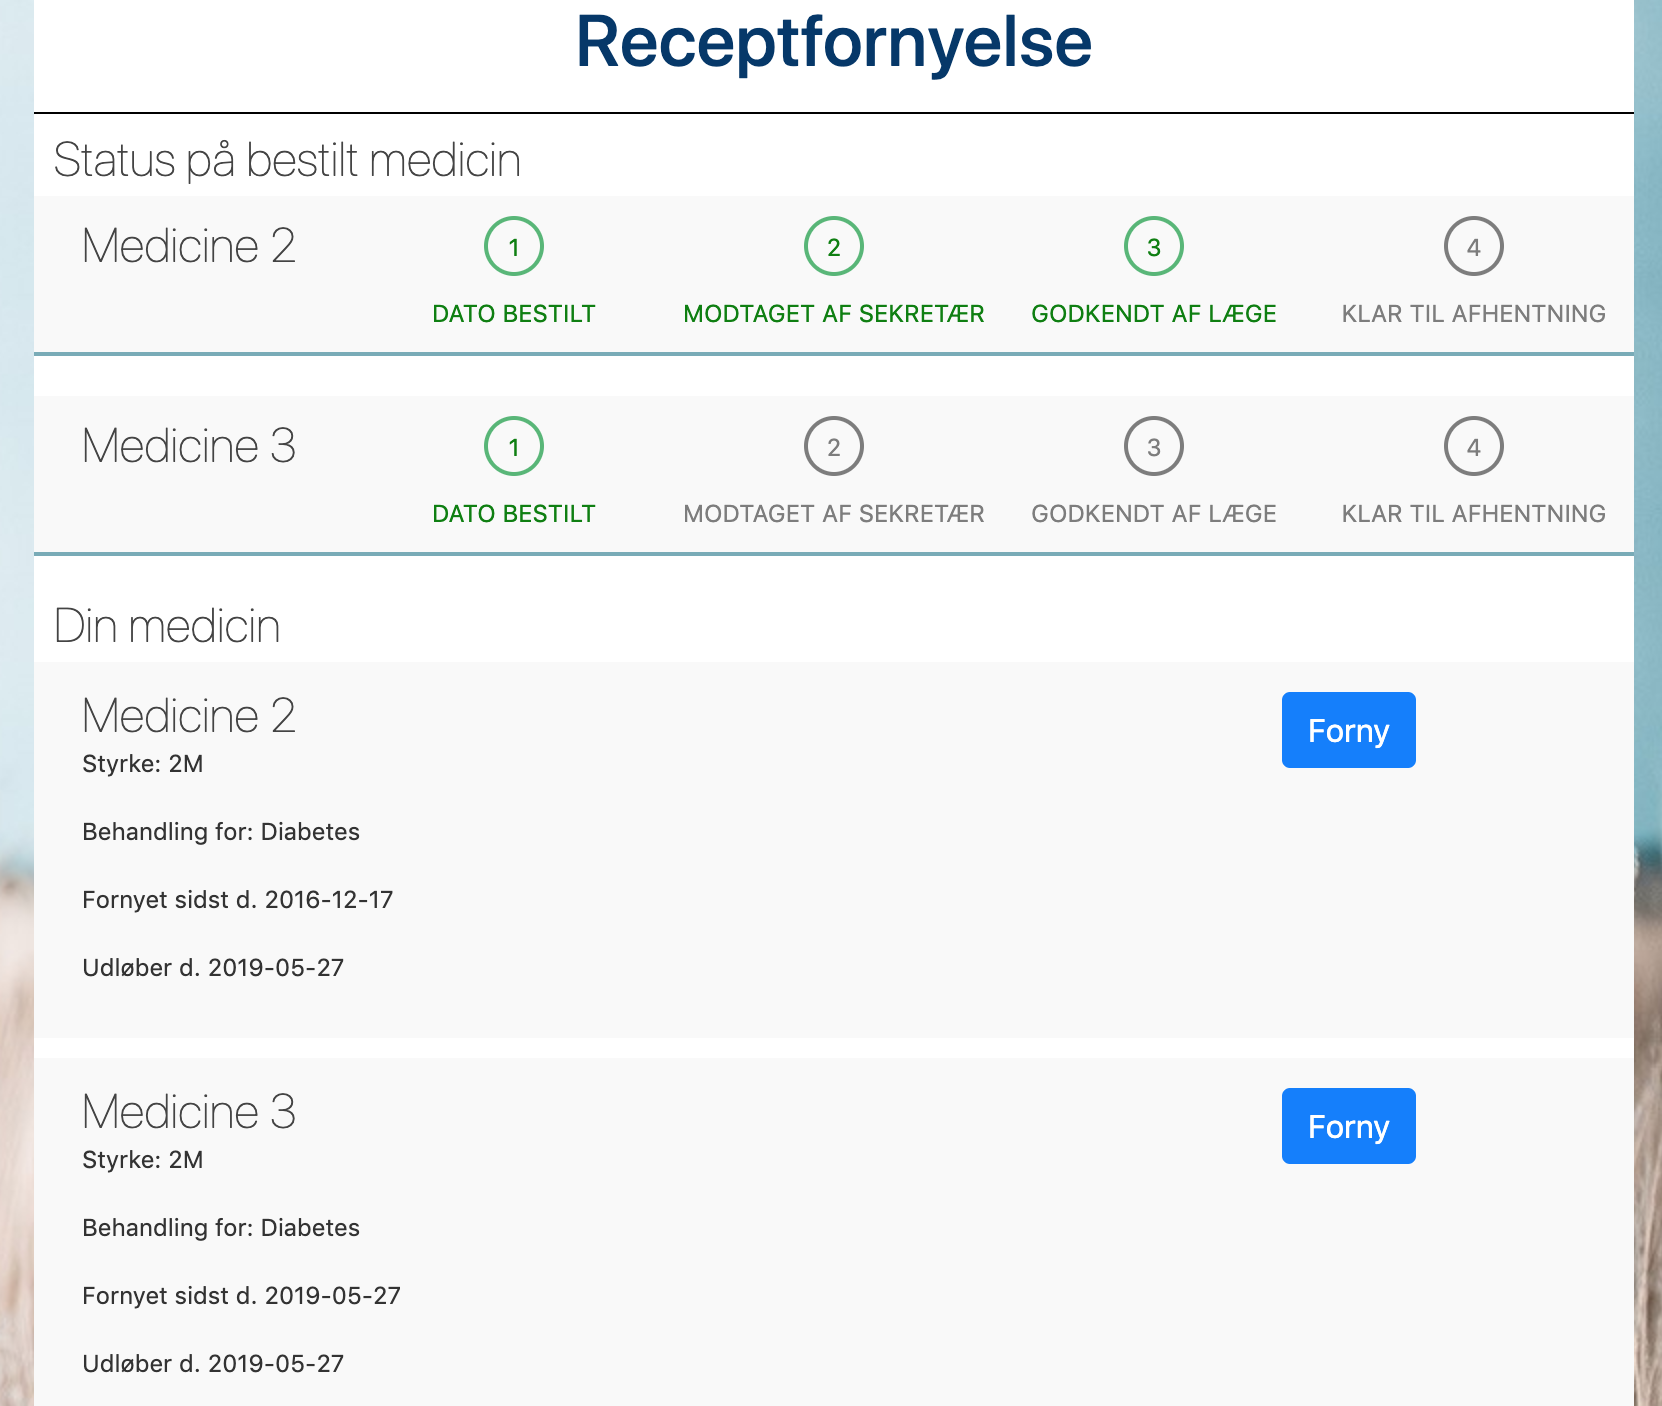
\includegraphics[width=0.49\linewidth]{Materials/Prototype/ReceptfornyelseFornyet}
	\caption{tv. ses recepterne før fornyelse. th. ses recepterne efter 'Medicine 3' fornyelse}
\end{figure}
\todo{Medicin kort?}
\subsection{Known shortcommings}
Der er endnu ikke implementeret business logic til at sørge for at recepten kun kan fornys når den er ved at udløbe, og den kan derfor fornyelse så ofte det ønskes.\\
Mange værdier er hard coded når der indsættes en ny recept gennem receptfornyelsen. Dette ville relativt nemt kunne løses ved at lave om på database modelen. Da dette er en prototype hvis formål er at illustrere en mulig løsning har dette ikke været en prioritet at løse. 